% -------------------------------------------------------------------------------- %

\begin{exercise}[18]

Zeigen Sie:

\begin{enumerate}[label = \alph*.]
    \item $\neg (p_1 \land p_2) \Leftrightarrow \neg p_1 \lor \neg p_2$.
    \item Für alle Formeln $A$ und $B$ gilt $\neg (A \land B) \Leftrightarrow \neg A \lor \neg B$.
\end{enumerate}

\end{exercise}

% -------------------------------------------------------------------------------- %

\begin{solution}

\phantom{}

\begin{enumerate}[label = \alph*]

    \item Die folgende Wahrheitstafel zeigt, dass die \enquote{rhs} und \enquote{lhs} äquivalent sind. \\

    \begin{tabular}{|c|c|c|c|}
        \hline
        $p_1$ & $p_2$ & $\neg (p_1 \land p_2)$ & $\neg p_1 \lor \neg p_2$ \\
        \hline
        $1$ & $1$ & $0$ & $0$ \\
        \hline
        $1$ & $0$ & $1$ & $1$ \\
        \hline
        $0$ & $1$ & $1$ & $1$ \\
        \hline
        $0$ & $0$ & $1$ & $1$ \\
        \hline
    \end{tabular}

    \item GEHT DAS AUCH?! \\

    \begin{tabular}{|c|c|c|c|}
        \hline
        $A$ & $B$ & $\neg (A \land B)$ & $\neg A \lor \neg B$ \\
        \hline
        $1$ & $1$ & $0$ & $0$ \\
        \hline
        $1$ & $0$ & $1$ & $1$ \\
        \hline
        $0$ & $1$ & $1$ & $1$ \\
        \hline
        $0$ & $0$ & $1$ & $1$ \\
        \hline
    \end{tabular}

\end{enumerate}

\end{solution}

% -------------------------------------------------------------------------------- %

\begin{solution}

\phantom{}

\begin{enumerate}[label = \alph*.]

    \item Eine (vielleicht) etwas übersichtlichere Wahrheitstafel.

    \begin{align*}
        \begin{array}{cccccccccc}
            \neg & (p_1 & \land & p_2) & \iff & \neg & p_1 & \lor & \neg & p_2 \\
            \hline
            2 & 0 & 1 & 0 & 3 & 1 & 0 & 2 & 1 & 0 \\
            \hline
            F & W & W & W & W & F & & F & F & \\
            W & W & F & F & W & F & & W & W & \\
            W & F & F & W & W & W & & W & F & \\
            W & F & F & F & W & W & & W & W &
        \end{array}
    \end{align*}

    \item Wir wählen zwei beliebige aussagenlogische Formeln $A$ und $B$.
    Sei $\mathcal{F}(V)$ die Menge aller Formeln über der Variablenmenge $V$.
    Sei nun $V$ eine Variablenmenge, sodass $A \in \mathcal{F}(V)$ und $B \in \mathcal{F}(V)$ und $\Bbraces{p_1, p_2} \subseteq V$ und $p_1 \neq p_2$.
    Wir definieren

    \begin{align*}
        g:
        V \to \mathcal{F}(V):
        x \mapsto
        \begin{cases}
            A, & x = p_1 \\
            B, & x \neq p_1
        \end{cases}.
    \end{align*}

    \includegraphicsboxed{../../../Fundament-LaTeX/images/LGM/LGM - Bemerkung II.1.15.png}

    \begin{figure}[h!]
        \begin{boxedin}
            \begin{center}
                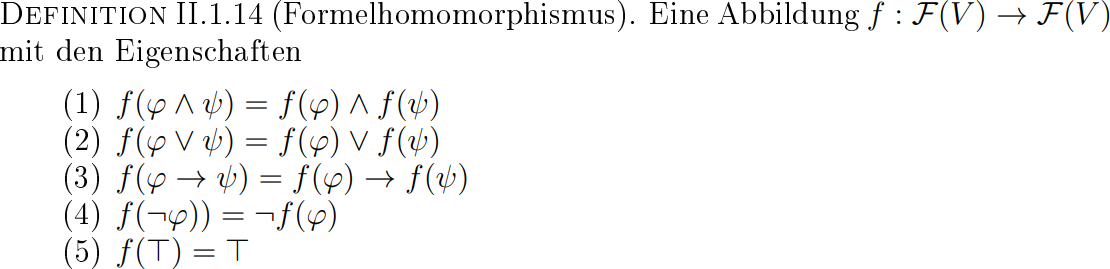
\includegraphics[width = 0.75 \textwidth]{../../../Fundament-LaTeX/images/LGM/LGM - Definition II.1.14.1 (Formelhomomorphismus).png} \\
                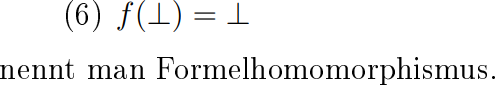
\includegraphics[width = 0.125 \textwidth]{../../../Fundament-LaTeX/images/LGM/LGM - Definition II.1.14.2 (Formelhomomorphismus).png}
            \end{center}
        \end{boxedin}
    \end{figure}

    Nach Bemerkung II.1.15 im Skriptum, lässt sich $g$ eindeutig zu einem Formelhomomorphismus (vgl. Definition II.1.14) $f:\mathcal{F}(V) \to \mathcal{F}(V)$ fortsetzen.

    \includegraphicsboxed{../../../Fundament-LaTeX/images/LGM/LGM - Satz II.1.9.png}

    Aus (a) und Satz II.1.9. wissen wir, dass $\varphi := \neg (p_1 \land p_2) \leftrightarrow \neg p_1 \lor \neg p_2$ eine Tautologie ist.

    \includegraphicsboxed{../../../Fundament-LaTeX/images/LGM/LGM - Satz II.1.16.png}

    Mit Satz II.1.16 ist auch $f(\varphi)$ eine Tautologie.

    \begin{align*}
        f(\varphi) = \neg (A \land B) \leftrightarrow \neg A \lor \neg B
    \end{align*}

    Mit Satz II.1.9 gilt die zu zeigende Äquivalenz.

\end{enumerate}

\end{solution}

% -------------------------------------------------------------------------------- %
